\chapter{实验设计及结果分析}\label{chap:Result}

本章节主要介绍基于前述算法设计的LS\_NRA求解工具的实验结果,并基于此对其性能进行了分析。本章节主要可以分为三个部分:首先我介绍实验安排和实验条件,包括测试样例、比较方法、运行环境等;然后我给出LS\_NRA与其他主流求解器的求解个数与时间对比;最后我对前几章提出的策略设计了消融实验,确保本文介绍的算法的有效性。

\section{实验设置}
\subsection{测试样例}
本工作选取SMT-LIB\footnote{\url{https://smt-lib.org/}}中QF\_NRA理论作为测试样例。测试样例大多包含来自工业问题的实例,我介绍其中一些类别如下:

\begin{itemize}
    \item \textbf{2019-ezsmt\cite{SusmanL16, ShenL18}:} 该类别来自一种处理non-tight程序的工具EZSMT+。
    \item \textbf{20170501-Heizmann\cite{Heizmann}:} 该类别来自Ultimate程序分析框架的一个组件,主要用于基于约束的不变式合成。
    \item \textbf{20200911-Pine\cite{Pine}:} 该类别来自名为Pine的工具,主要用于检查循环不变式的归纳性。
    \item \textbf{LassoRanker\cite{LeikeH15, HeizmannHLP13, Lasso3}:}该类别来自一种使用秩函数来分析Lassoshaped程序终止性的工具,所含样例都是多线性(multilinear)约束。
    \item \textbf{UltimateAutomizer:}该类别产生自基于自动机的软件模型检查工具,是Ultimate软件分析工具的一个组件。
\end{itemize}

\textbf{样例选择:} 在SMT-LIB中,每一个测试样例会标注标签(label),即SAT、UNSAT或UNKNOWN,用来表示是否被其他的求解器求解。由于局部搜索算法只能用来求解可满足的样例,因此我首先使用主流的SMT求解器(Z3、CVC5、Yices)来被证明为UNSAT的样例,最终留下潜在的可满足样例作为本文的最终测试样例。最终我收集了6216个测试样例。


\subsection{实验方法}
 \textbf{实验环境:} 所有实验都在一台配备有Intel Xeon Platinum 8153(2.00GHz)和2048G RAM 的服务器上进行,系统为Centos 7.7.1908。每一个样例设置的时间限制为20分钟(和SMT比赛相同),内存限制为30GB。由于我的工具LS\_NRA是基于Z3实现的,我保留了默认的随机数设置,来确保与原版Z3求解器对比的公平性。

 \textbf{比较对象:} 我选择目前SMT-COMP非线性赛道表现最优的三个求解器(Z3\cite{MouraB08}、CVC5\cite{BarbosaBBKLMMMN22}、Yices\cite{Dutertre14})作为基准算法。这三个求解器主要使用CDCL(T)和MCSAT等完备算法处理非线性理论,因此是和本文这类非完备算法作比较的良好对象。

\textbf{比较方法:} 对于每一个样例,求解器可以输出求解结果(SAT、UNSAT或TIMEOUT)、运行时间和内存占用等信息。我收集每一个求解器的信息用于后面的结果展示。除此之外,我对主流求解器均采用默认设置,比如默认不采用增量式求解,全部使用串行方法等。

\section{LS\_NRA求解NRA样例的能力}
我在表\ref{tab:experiment}中展示了我的工具LS\_NRA与其他主流SMT求解器的性能对比。在全部样例上,LS\_NRA求解出了最多的样例,超过第二名Z3求解器约100个。在单独的样例上,LS\_NRA与主流完备算法求解器存在不同的优势,我根据类别介绍如下:
\begin{itemize}
    \item \textbf{高次多项式约束:} 
    LS\_NRA在高次多项式约束上有很好的表现,比如20161105-Sturm-MBO类别。该类别包含一个高次多项式约束等式,并且要求所有变量只能取正值,可以理解为判断一个给定的多项式是否存在全正值解。比如约束$F = x^100 + y^ 223 + x^45 y^23 \wedge x > 0 \wedge y > 0$。基于CDCL(T)和MCSAT的主流求解器一般使用柱形代数分解(CAD)用来产生学习子句,其复杂度与多项式的次数呈现双指数关系,因此在多项式投影阶段存在巨大的资源消耗。对于局部搜索算法而言,每次迭代仅需要更改一个变量,将其他变量视为常数,因此将多元高次多项式转变为一元高次多项式来处理。在实际求解效果中,LS\_NRA求解了84个样例,首次突破了主流求解器在该类别上的零求解纪录。

    \item \textbf{多线性(multilinear)约束:}LS\_NRA的另一个优势在于LassoRanker类别为代表的多线性约束,即只包含不同变量乘积的多项式约束,如$x y + y z + x z \leq 3$。CVC5一般采用增量线性化方法将这种约束抽象成线性约束,然后调用线性约束求解器进行求解,效果在该样例上取得了最好。LS\_NRA在该类别上求解了284个样例,仅次于CVC5,主要原因来自于对线性不等式可行域的特殊处理。
\end{itemize}

对于某些样例(2019-ezsmt、UltimateAutomizer)来说,LS\_NRA的求解效果不如主流求解器。这类约束一般包含复杂低次约束,主流求解器可以通过单元传播等推理技术快速排除不可行赋值,而局部搜索算法往往需要多次迭代采样才能找到可行胞腔,因此在求解效果上稍有差距。

除此之外,我的算法和Z3、CVC5有很大的互补性。根据表\ref{tab:experiment},一共有来自不同类别共148个样例仅仅可以使用局部搜索算法(LS\_NRA)求解,而非Z3、CVC5、Yices等完备算法。更具体来说,有291个样例可以被局部搜索求解而非Z3,有378个样例可以被局部搜索求解而非CVC5。表格最后一栏给出了只能够通过LS\_NRA求解,而不能被Z3、CVC5、Yices任意求解器求解的样例个数。可以看出,LS\_NRA在求解器中有很好的互补性,能够处理一些主流求解器无法处理的样例。

\begin{table*}[]
    \centering
    \resizebox{\linewidth}{!}{
        \begin{tabular}{c | c | c | c | c | c | c}
            \hline
            类别 & 个数 & Z3 & CVC5 & Yices & LS\_NRA (本文) & 单独求解 \\\hline
            20161105-Sturm-MBO & 120 & 0 & 0 & 0 & 84 & 84 \\
            20161105-Sturm-MGC & 2 & 2 & 0 & 0 & 0 & 0 \\
            20170501-Heizmann & 60 & 2 & 1 & 0 & 6 & 5 \\
            20180501-Economics-Mulligan & 93 & 93 & 89 & 91 & 87 & 0 \\
            2019-ezsmt & 61 & 56 & 50 & 52 & 18 & 0 \\
            20209011-Pine & 237 & 234 & 199 & 235 & 224 & 0 \\
            20211101-Geogebra & 112 & 110 & 91 & 99 & 100 & 0 \\
            20220314-Uncu & 74 & 69 & 62 & 70 & 70 & 0 \\
            LassoRanker & 351 & 167 & 305 & 122 & 284 & 15 \\
            UltimateAtomizer & 48 & 35 & 35 & 39 & 26 & 2 \\
            hycomp & 492 & 307 & 225 & 227 & 270 & 17 \\
            kissing & 42 & 33 & 17 & 10 & 33 & 2 \\
            meti-tarski & 4391 & 4391 & 4343 & 4369 & 4356 & 0 \\
            zankl & 133 & 70 & 58 & 58 & 99 & 26 \\\hline
            总和 & 6216 & 5569 & 5475 & 5372 & 5657 & 151 \\\hline
        \end{tabular}
        }
        \bicaption{LS\_NRA和其他SMT求解器的求解能力对比。} {Comparison of LS\_NRA and other SMT solvers.}
\label{tab:experiment}
\end{table*}

我在图\ref{fig:scatter}中描绘了LS\_NRA与Z3(左上)、CVC5(右上)、Yices(左下)求解时间对比的散点图。图中每一个点的横坐标代表了求解该样例LS\_NRA所需要的时间,纵坐标表示了其他求解器的求解时间,虚线则说明二者在该问题上消耗的求解时间一致。可以看到与CVC5相比,大多数散点在虚线以上,说明对于大部分样例的求解LS\_NRA更有优势。除此之外,三个散点图中均有不少样例分布在虚线以上,这说明了对于某些样例而言,局部搜索算法有很强的针对性。


\begin{figure*}[t]
    \centering
    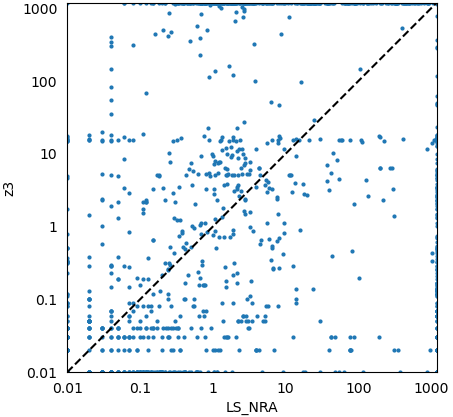
\includegraphics[width=0.45\columnwidth]{Img/scatter_z3.png}\qquad
    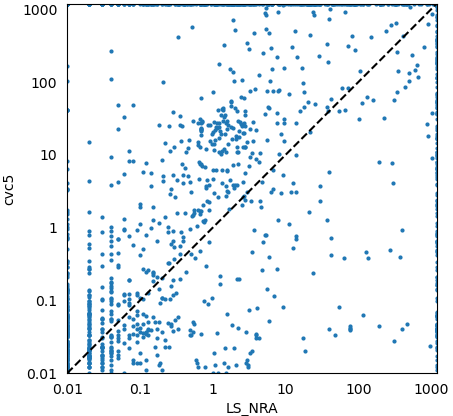
\includegraphics[width=0.45\columnwidth]{Img/scatter_cvc5.png}\qquad
    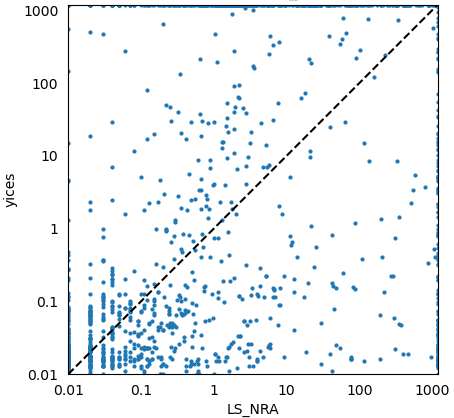
\includegraphics[width=0.45\columnwidth]{Img/scatter_yices.png}\qquad
    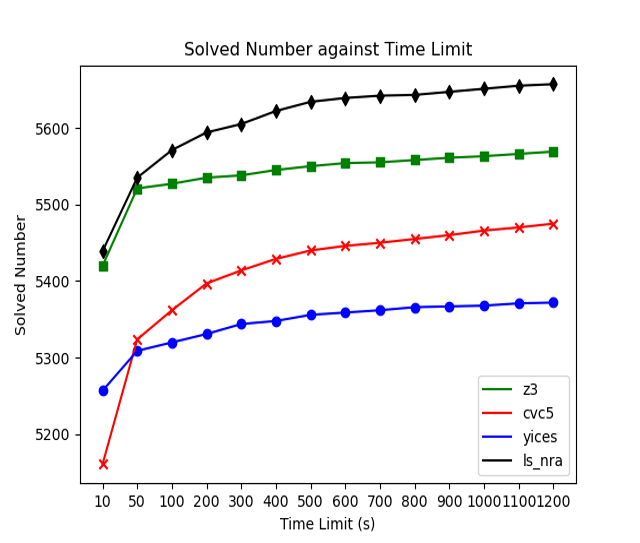
\includegraphics[width=0.45\columnwidth]{Img/time_solver.png}
    \bicaption{LS\_NRA与Z3 (左上)、CVC5 (右上)、Yices (左下)求解时间对比。不同求解器在不同限定时间内求解个数比较(右下)。} {Comparison of LS\_NRA and Z3 (upper left), CVC5 (upper right), Yices (lower left) solving time. Comparison of number of solutions found by different solvers in different time (lower right).}
\label{fig:scatter}
\end{figure*}

我还参考了不同求解器的求解时间对比,如图\ref{fig:scatter}右下图所示。可以看出,几乎在任何的限制时间内,局部搜索算法的求解数量都是最多的,这说明局部搜索算法对计算时间的要求相对较低,程序迭代速度较快。随着求解时间的增加,局部搜索算法的求解数量增长速度远远快于其他求解器,这说明在充足的时间内,更多的样例可以通过多次迭代找到邻近的可行解。相较于完备算法而言,局部搜索算法的另一优势是可以在任意时间内返回质量足够好(接近可满足赋值)的解,为后续其他算法提供了更好的初始解。



\section{和其他局部搜索工作的对比}
我还讨论了LS\_NRA与以往局部搜索工作的对比。在\cite{multilinear}考虑的979个多线性样例中,LS\_NRA可以求解826个,略小于前序工作的891个。这种微弱的差异主要来自于\cite{multilinear}更高效的实现,考虑到其工作只需要考虑有理数赋值,而非代数数,因此在数据结构设计和参数优化上更有针对性。在\cite{LiXZ23}考虑的2736个样例中,我的方法可以求解2589个,高于前序工作的2246个。事实上,我不仅比局部搜索算法求解的个数要多,也要比前面工作用于对比的其他求解器个数还要多。我注意到\cite{LiXZ23}使用了不同的计算软件(比如Maple),并且在不同机器上测试,因此数据可能略有误差。

% \begin{figure*}[t]
%     \centering
%     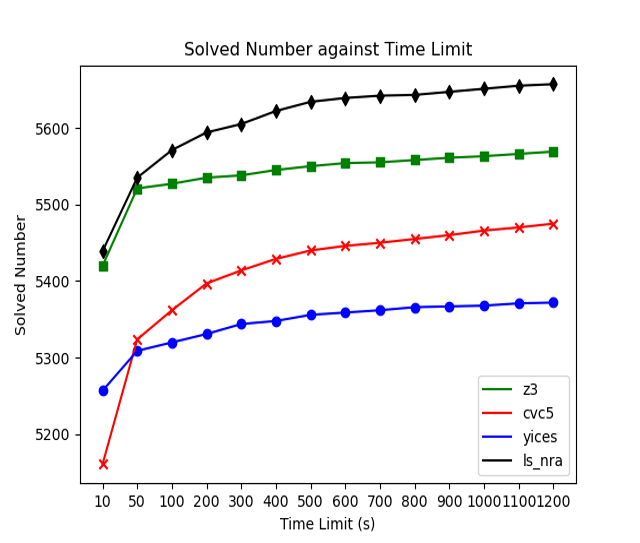
\includegraphics[width=0.65\columnwidth]{Img/time_solver.png}
%     \bicaption{LS\_NRA与Z3、CVC5在不同时间求解个数对比。}{Comparison of LS\_NRA and Z3, CVC5 solving number in different time.}
% \label{fig:time}
% \end{figure*}

\section{消融实验1:变量分数增量式计算的影响}
本小节主要展示章节\ref{chap:method1}中提出的变量分数增量式计算对迭代加速的影响。我比较如下集中实现:基于边界的增量式计算(Incremental),不采用增量式计算的传统方法(Naive),以及传统方法但是限制每次考虑的子句数最大为45(Limit-45)。相关的结果如表格\ref{tab:incremental}所示。

我注意到不同实现方法的求解总数差异并不大,并且主要集中在LassoRanker类别上。LassoRanker样例因为子句数量的庞大一般需要比较长时间求解,因此不同实现方法对迭代速度的影响十分重要。通过对比求解时间可以看出对于一个特定的问题而言,Naive和Limit-45的方法基本需要消耗2-10倍于Incremental方法的时间,具体的倍数在不同问题上有所不同。

图\ref{fig:scatter_inc}显示了在使用和不使用增量式计算的情况下,局部搜索求解单个样例所需的整体时间(左图)和每次迭代所需时间(右图)。每一个点表示一个测试样例,横纵坐标分别代表了使用和不使用增量式计算下的求解时间。根据散点图可知,绝大多数点分布在虚线以上,这意味着增量式计算在绝大多数样例上增量式计算可以起到提高求解速度的作用。右图可以看出增量式计算在每次迭代的时间上也有所提升。另一方面,我统计得出基于边界的计算方法往往需要更少的迭代步数,这说明新的计算方法成功规避了传统计算大量同类操作的发生。


图\ref{fig:time_inc}显示了是否使用增量式计算在不同时间限制下的求解个数。对于1200秒的限制来说,是否使用增量式计算对求解个数的影响并不明显,但是在更少的求解时间时(300秒以下),更多的计算资源消耗在了实根隔离和可行域计算上,因此在迭代中缓存这些昂贵的信息尤为重要。在求解时间为10秒的条件下,二者的差距有150个以上,这说明在运行初期大量时间被用于计算变量的可行域区间,因此增量式缓存机制尤为重要。

\begin{figure*}[t]
    \centering
    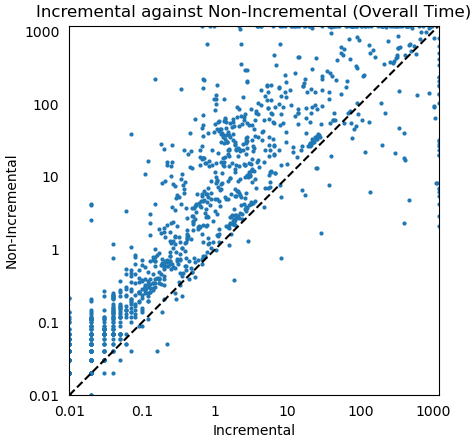
\includegraphics[width=0.45\columnwidth]{Img/scatter_inc_ninc_time.png}\qquad
    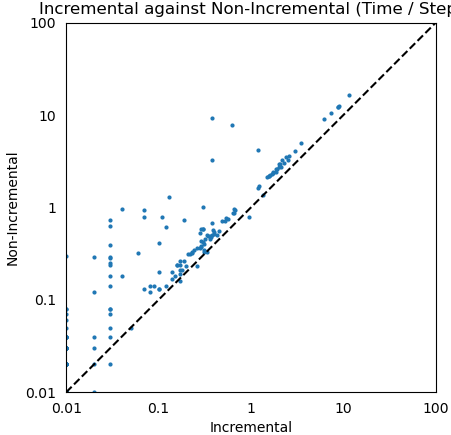
\includegraphics[width=0.45\columnwidth]{Img/scatter_inc_ninc_pertime.png}
    \bicaption{增量式计算对整体求解时间和单步迭代时间的影响。}{Empact of incremental calculation on total solving time and per-iteration time.}
\label{fig:scatter_inc}
\end{figure*}
\begin{figure*}[t]
    \centering
    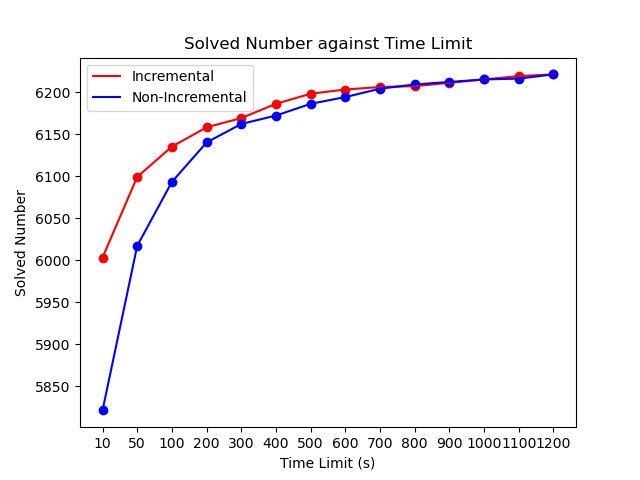
\includegraphics[width=0.7\columnwidth]{Img/time_inc.png}
    \bicaption{LS\_NRA使用增量式计算在不同时间下求解的个数。}{Number of solutions found by LS\_NRA with incremental calculation in different time.}
\label{fig:time_inc}
\end{figure*}


\begin{table*}[]
    \centering
    \resizebox{0.8\linewidth}{!}{
        \begin{tabular}{c | c | c | c | c}
            \hline
            类别 & 个数 & Incremental & Naive & Limit-45 \\\hline
            20161105-Sturm-MBO & 120 & 84 & 84 & 84 \\\hline
            20161105-Sturm-MGC & 2 & 0 & 0 & 0 \\\hline
            20170501-Heizmann & 60 & 6 & 5 & 5 \\\hline
            20180501-Economics-Mulligan & 93 & 87 & 88 & 88 \\\hline
            2019-ezsmt & 61 & 18 & 19 & 15 \\\hline
            20209011-Pine & 237 & 224 & 221 & 221 \\\hline
            20211101-Geogebra & 112 & 100 & 99 & 99 \\\hline
            20220314-Uncu & 74 & 70 & 70 & 70 \\\hline
            LassoRanker & 351 & 284 & 262 & 267 \\\hline
            UltimateAtomizer & 48 & 26 & 26 & 26 \\\hline
            hycomp & 492 & 270 & 257 & 257 \\\hline
            kissing & 42 & 33 & 32 & 33 \\\hline
            meti-tarski & 4391 & 4356 & 4345 & 4345 \\\hline
            zankl & 133 & 99 & 98 & 98 \\\hline
            总和 & 6216 & 5657 & 5606 & 5608 \\\hline
        \end{tabular}
        }
        \bicaption{增量式计算对算法的影响。} {Impact of incremental calculation on algorithm.}
\label{tab:incremental}
\end{table*}

\section{消融实验2:等式约束松弛的影响}
本小节主要展示章节\ref{chap:method2}中介绍的等式约束松弛对整体算法的影响。我给出以下三种版本:使用等式松弛机制(Relaxation),不使用等式松弛但优先选取低复杂度的赋值(Threshold),不使用等式松弛并且不考虑赋值复杂度(NoOrder)。相关结果在表\ref{tab:relaxation}中展示。

我可以看到,在整体求解效果上,使用等式松弛机制的效果最好,其次是考虑赋值复杂度和传统方法。三者的主要差距在于hycomp样例,该样例来自于混成自动机的分析和验证,包含了大量的等式约束,并且结果往往涉及无理数赋值。等式松弛技术可以暂缓对于等式约束可满足的处理,进而将计算资源放在更容易处理的严格不等式上,求得近似解后再迭代到最近的精确解。考虑赋值复杂度的方法则会规避一些复杂的有理数赋值,提高每次迭代的速度,进而在更短时间内求解更多的样例。

经过统计,有1109个样例在实际运行中涉及到了等式松弛,使用松弛技术后可以在1200秒时间限制内求解出96个以前求解超时的样例。其中,对于一些等式约束非常复杂的样例,比如hycomp类别下的ball\_count样例,使用等式松弛技术后可以在110秒内成功求出可行解。我还统计了等式松弛技术中恢复阶段所需时间和占总迭代时间比例的规律,如图\ref{fig:restore2}所示。结果表明绝大部分样例(926个)可以在很短时间内(< 0.1秒)的恢复阶段在0.1秒内完成,超过100秒的样例很少,说明我的松弛算法可以在很短时间内迅速找到精确解。同时,我还统计了恢复阶段耗时占整体求解时间的比例分布,大约66\%的样例恢复阶段耗时占总时间比例小于10\%,但仍然存在部分难以处理的样例可能很难找到精确解。这部分样例一般存在于多个变量构成的等式方程组中,并且大部分变量的赋值均采用无理数,因此本文提出的基于单个约束的松弛方法可能无法很好地处理这类问题。

\section{本章小结}
本章节通过设计实验,深入评估了LS\_NRA工具的求解性能和策略有效性。首先,我对比了LS\_NRA和其他主流SMT求解器(Z3、CVC5、Yices)在SMT-LIB上的求解个数和求解时间,方法表明LS\_NRA对于高次约束具有优势。然后,我设计消融实验测试了基于边界的可行域缓存机制和等式松弛机制对整体求解效果的影响,实验表明二者均对算法的求解能力有所提升。

\begin{figure*}[t]
    \centering
    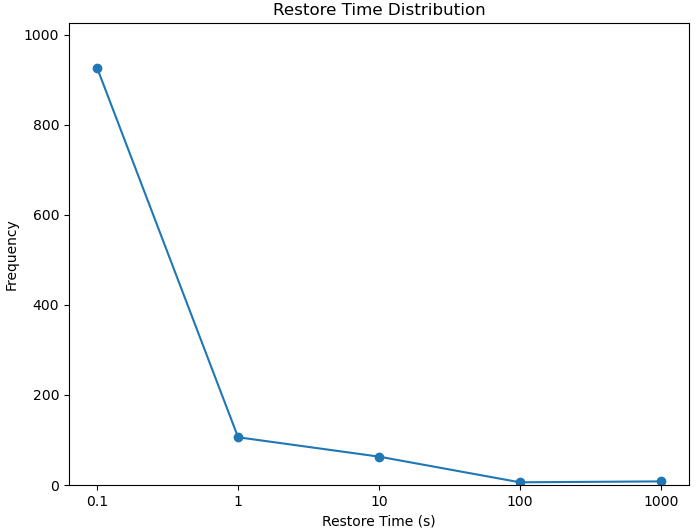
\includegraphics[width=0.45\columnwidth]{Img/restore_time.png}\qquad
    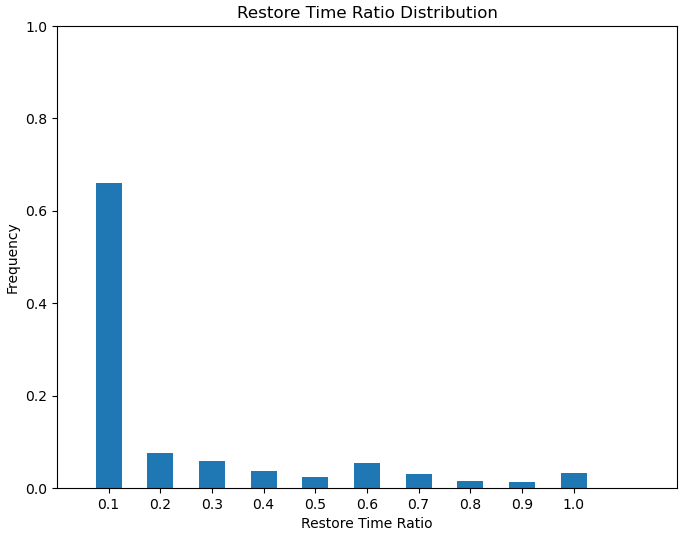
\includegraphics[width=0.45\columnwidth]{Img/restore_ratio.png}
    \bicaption{左图:松弛解恢复时间分布。右图:松弛解恢复时间占总时间比例。}{Left: Distribution of restoration time. Right: Ratio of restoration time to total time.}
\label{fig:restore2}
\end{figure*}

\begin{table*}[]
    \centering
    \resizebox{0.9\linewidth}{!}{
        \begin{tabular}{c | c | c | c | c}
            \hline
            类别 & 个数 & Relaxation & Threshold & NoOrder \\\hline
            20161105-Sturm-MBO & 120 & 84 & 85 & 84 \\\hline
            20161105-Sturm-MGC & 2 & 0 & 0 & 0 \\\hline
            20170501-Heizmann & 60 & 6 & 9 & 3 \\\hline
            20180501-Economics-Mulligan & 93 & 87 & 89 & 86 \\\hline
            2019-ezsmt & 61 & 18 & 18 & 18 \\\hline
            20209011-Pine & 237 & 224 & 220 & 220 \\\hline
            20211101-Geogebra & 112 & 100 & 100 & 92 \\\hline
            20220314-Uncu & 74 & 70 & 70 & 70 \\\hline
            LassoRanker & 351 & 284 & 283 & 278 \\\hline
            UltimateAtomizer & 48 & 26 & 24 & 19 \\\hline
            hycomp & 492 & 270 & 204 & 158 \\\hline
            kissing & 42 & 33 & 31 & 27 \\\hline
            meti-tarski & 4391 & 4356 & 4348 & 4355 \\\hline
            zankl & 133 & 99 & 99 & 99 \\\hline
            总和 & 6216 & 5657 & 5580 & 5509 \\\hline
        \end{tabular}
        } 
        \bicaption{等式约束松弛对算法的影响。} {Impact of relaxation on algorithm.}
\label{tab:relaxation}
\end{table*}